\documentclass[12pt]{article}

\usepackage{adjustbox}
\usepackage{amsmath}
\usepackage{mathpazo}
\usepackage{color}
\usepackage[utf8]{inputenc}
\usepackage{graphics}
\usepackage[colorlinks,urlcolor=blue]{hyperref}
\usepackage{standalone}
\usepackage{svg}
\usepackage{tikz}
\usepackage{tikz-3dplot}

\usetikzlibrary{decorations.pathreplacing,calligraphy}

\textheight=20cm 
\textwidth=15cm
\oddsidemargin=1.0cm

\newcommand{\pmat}[1]{\begin{pmatrix}#1\end{pmatrix}}

\begin{document}

\begin{titlepage}
    \begin{center}
        \vspace*{0.1\paperheight}
        
\includegraphics[width=0.20\textwidth]{logo.png} \par
        {\huge CartPole: dynamics and control \par}
        \vspace{\stretch{0.05}}
        {\Large Robotics Group \par}
        \vspace*{\fill}
    \end{center}
 \end{titlepage}

\section{Dynamics}

CartPole is a classic control problem:
cart moving along a horizontal line with freely hanging pendulum (metal pole) attached to it.
Device is controlled with cart acceleration (stepper motor as drive),
the goal is to bring up the pendulum to unstable equilibrium position and maintain it there.

\subsection{Linear CartPole}

A cart with mass $m_c$ moves along the $x$-axis, so its center $C$ has coordinates $(x, 0)^T$.
A pole with mass $m_p$ is attached to the cart with a hinge at point $C$,
and rotates around with viscous friction.
The pole's center of mass is at $P$, moment of inertia is $I_p$.
The angle of rotation is denoted as $\theta$, measured counterclockwise from the axis $-y$.
A force $f_x$ is applied to the cart and the force of gravity $g$ acts on the pole.

\begin{center}
    \begin{adjustbox}{width=0.7\textwidth}
        \documentclass[dvisvgm,tikz]{standalone}

\usepackage{amsmath}
\usepackage{mathpazo}
\usepackage[utf8]{inputenc}
\usepackage{graphics}
\usepackage[colorlinks,urlcolor=blue]{hyperref}
\usepackage{standalone}
\usepackage{svg}
\usepackage{tikz}

\usetikzlibrary{arrows.meta,decorations.pathreplacing,calligraphy}
\special{background White}

\begin{document}
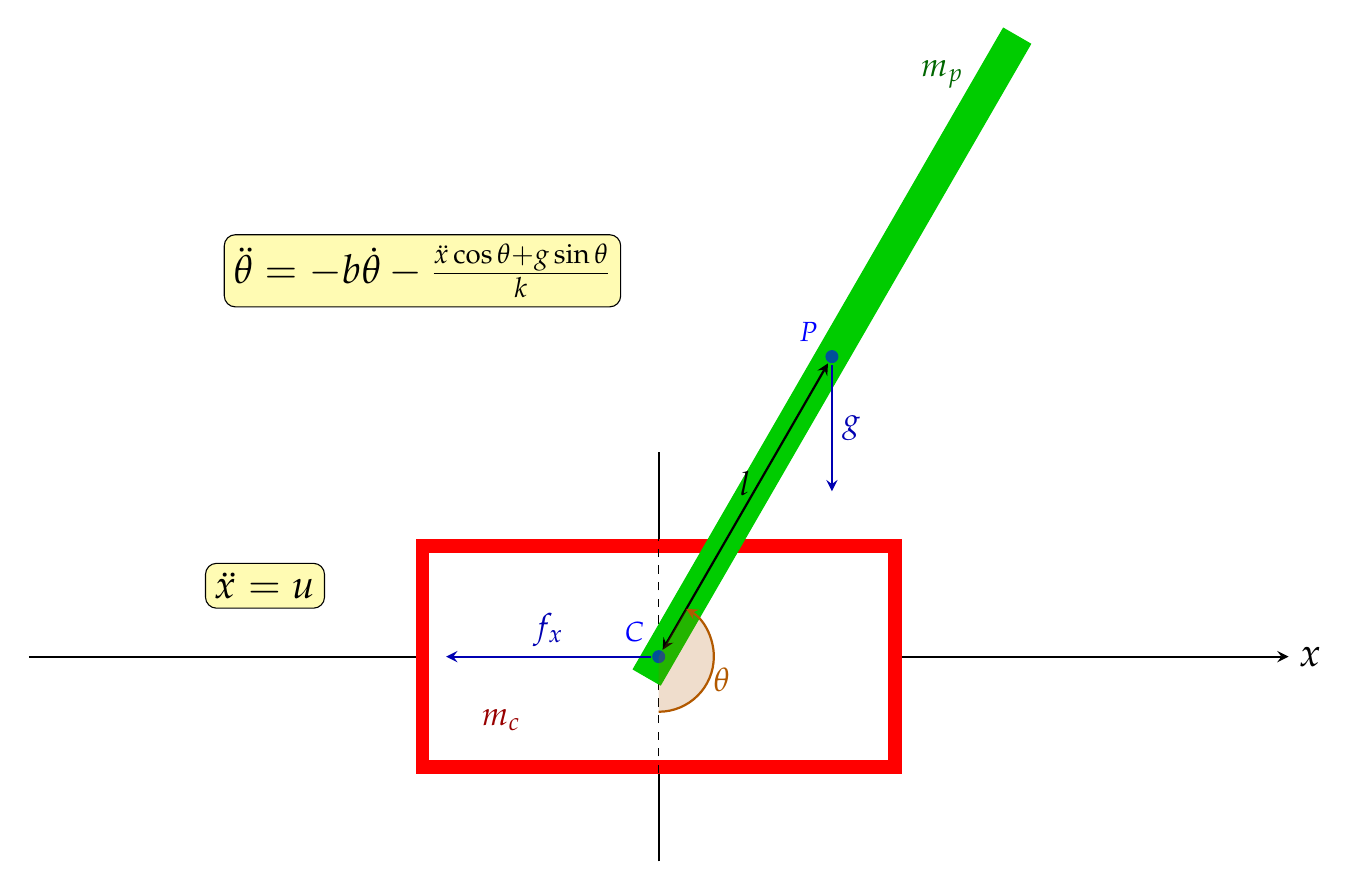
\begin{tikzpicture}[>=stealth]
    % world
    \draw[->, thick] (-1,3.1) -- (15,3.1) node[right] {\Large $x$};
    \draw[-, thick] (7,0.5) -- (7,5.7);

    % hull
    \filldraw[red!100!black, fill=white, line width=5] (4.0,1.7) rectangle (10.0,4.5);

    % y axis help
    \draw[-, dashed] (7,1.2) -- (7,5.0);

    % stick
    \begin{scope}[rotate around={150:(7, 3.1)}]
        \filldraw[green!80!black, fill=green!80!black] (6.8, 3.4) rectangle (7.2, -6);

        % C
        \node[circle, fill=blue, opacity=0.6, scale=0.5, label={above left:{\textcolor{blue}{$C$}}}] at (7, 3.1) {};

        % P
        \node[circle, fill=blue, opacity=0.6, scale=0.5, label={above left:{\textcolor{blue}{$P$}}}] at (7, -1.3) {};

        % l
        \draw[<->, thick, black] (7,3) -- (7, -1.2) node[midway,above] {\large $l$};
    \end{scope}

    % f_x
    \draw[<-, thick, blue!70!black] (4.3,3.1) -- (6.9, 3.1) node[midway,above] {\large $f_x$};

    % g
    \draw[->, thick, blue!70!black] (9.2, 6.81) -- (9.2, 5.2) node[midway,right] {\large $g$};

    % \theta
    \draw[->, thick, orange!70!black] (7, 2.4) arc [start angle=-90, end angle=60, radius=0.7];
    \fill[->, opacity=0.2, orange!70!black] (7, 3.1) -- (7, 2.4) arc [start angle=-90, end angle=60, radius=0.7];
    \draw[thick, orange!70!black] (7.8, 2.8) node {\large $\theta$};

    % m_C
    \draw[red!60!black] (5, 2.3) node {\large $m_c$};

    % m_P
    \draw[green!40!black] (10.6, 10.5) node {\large $m_p$};

    % formula
    \draw (4,8) node[fill=yellow!30, draw, rounded corners] {\Large $\ddot{\theta} = -b\dot{\theta} -\frac{\ddot{x} \cos \theta + g \sin \theta}{k}$};
    \draw (2,4) node[fill=yellow!30, draw, rounded corners] {\Large $\ddot{x} = u$};
\end{tikzpicture}
\end{document}

    \end{adjustbox}
\end{center}

\begin{align}
    & C = \pmat{x                 \\ 0}  & &\dot{C} = \pmat{\dot{x} \\ 0} \nonumber \\
    & P = \pmat{x + l \sin \theta \\ - l \cos \theta} & &\dot{P} = \pmat{\dot{x} + l \dot{\theta} \cos \theta \\ l \dot{\theta} \sin \theta}
\end{align}

The kinetic energy of the cart is
\begin{equation}
    T_c = \frac{1}{2} m_c \begin{Vmatrix}
        \dot{C}
    \end{Vmatrix}_2^2 = \frac{1}{2} m_c \dot{x}^2.
\end{equation}


Kinetic energy of the pendulum is the sum of translational and rotational energies
\begin{align}
    T_p & = T^t_p + T^r_p \nonumber \\
        & = \frac{1}{2} m_p \begin{Vmatrix}\dot{P}\end{Vmatrix}_2^2 + \frac{1}{2}I_p\dot{\theta}^2 \nonumber \\
        & = \frac{1}{2} m_p (\dot{x} + l \dot{\theta} \cos \theta )^2 + \frac{1}{2} m_p (l \dot{\theta} \sin \theta)^2 + \frac{1}{2}I_p\dot{\theta}^2 \nonumber \\
        & = \frac{1}{2} m_p \dot{x}^2 + m_p \dot{x} l \dot{\theta} \cos \theta + \frac{1}{2} \dot{\theta}^2 \left( m_p l^2  + I_p \right).
\end{align}

As a result energy of the whole system is following
\begin{align}
    T & = T_c + T_p \nonumber \\
      & = \frac{1}{2} m_c \dot{x}^2 + \frac{1}{2} m_p \dot{x}^2 + m_p \dot{x} l \dot{\theta} \cos \theta + \frac{1}{2} \dot{\theta}^2 \left( m_p l^2  + I_p \right) \nonumber \\
      & = \frac{1}{2} \dot{x}^2 (m_c + m_p) + m_p \dot{x} l \dot{\theta} \cos \theta + \frac{1}{2} \dot{\theta}^2 \left( m_p l^2  + I_p \right); \\
      & \nonumber \\
    U & = \underbrace{U_c}_{0} + U_p = -m_p gl \cos \theta.
\end{align}

To find the dynamics of system, let's use the Euler-Lagrange differential equation, where $L = T - U$, $q = (x, \theta)^T$ and $Q$ is the generalized force.
In our case, we have deal with two forces: motor force $f_x$ and viscous friction $f_{\theta}(\theta, \dot{\theta}) = -\mu \dot{\theta}$.

\begin{align*}
    Q &= \frac{d}{dt} \frac{dL}{d\dot{q}} - \frac{dL}{dq} \\ 
    Q &= \pmat{f_x \\ f_{\theta}}.
\end{align*}

As a result we get the following equations of motion
\begin{align}
    m_p \ddot{x} l \cos \theta + \ddot{\theta} \left(m_p l^2 + I_p\right) + m_p g l \sin \theta &= f_{\theta}(\theta, \dot{\theta}) \nonumber \\
    \ddot{x}(m_c + m_p) + m_p l \ddot{\theta} \cos \theta - m_p l \dot{\theta}^2 \sin \theta &= f_{x}.
\end{align}

A more detailed calculation is below
\begin{equation}
    L = \frac{1}{2} \dot{x}^2 (m_c + m_p) + m_p \dot{x} l \dot{\theta} \cos \theta + \frac{1}{2} \dot{\theta}^2 \left( m_p l^2  + I_p \right) + m_p gl \cos \theta.
\end{equation}

\begin{align*}
    \frac{dL}{d\theta}                                         & = - m_p \dot{x} l \dot{\theta} \sin \theta - m_p gl \sin \theta \\
    \frac{dL}{d\dot{\theta}}                                   & = m_p \dot{x} l \cos \theta + \left(m_p l^2 + I_p\right) \dot{\theta} \\
    \frac{d}{dt} \frac{dL}{d\dot{\theta}}                      & = m_p \ddot{x} l \cos \theta - m_p  \dot{x}  l \dot{\theta} \sin \theta + \left(m_p l^2 + I_p\right) \ddot{\theta}  \\
    \frac{d}{dt} \frac{dL}{d\dot{\theta}} - \frac{dL}{d\theta} & = m_p \ddot{x} l \cos \theta - m_p  \dot{x}  l \dot{\theta} \sin \theta + \left(m_p l^2 + I_p\right) \ddot{\theta} + m_p \dot{x} l \dot{\theta} \sin \theta + m_p gl \sin \theta \nonumber \\
                                                               & = m_p \ddot{x} l \cos \theta + \left(m_p l^2 + I_p\right) \ddot{\theta} + m_p g l \sin \theta \\
                                                               & \nonumber \\
    \frac{dL}{dx}                                              & = 0 \\
    \frac{dL}{d\dot{x}}                                        & = (m_c + m_p) \dot{x} + m_p l \dot{\theta} \cos \theta \\
    \frac{d}{dt} \frac{dL}{d\dot{x}}                           & = (m_c + m_p) \ddot{x} + m_p l \ddot{\theta} \cos \theta - m_p l \dot{\theta}^2 \sin \theta \\
    \frac{d}{dt} \frac{dL}{d\dot{x}} - \frac{dL}{dx}           & = (m_c + m_p) \ddot{x} + m_p l \ddot{\theta} \cos \theta - m_p l \dot{\theta}^2 \sin \theta. \\
\end{align*}

\subsection{Acceleration control}

Let's make the assumption that the motor can generate any force necessary for the cart to reach acceleration in $[-a, a]$ on a fixed cart velocity range.
This fact allows us to consider the cart acceleration as a control input and significantly simplify the equations of motion

\begin{align}
    \left(m_p l^2 + I_p\right) \ddot{\theta} &= f_{\theta}(\theta, \dot{\theta}) - m_p \ddot{x} l \cos \theta - m_p g l \sin \theta \nonumber \\
    \ddot{x}  &= u, \quad u \in [-a, a].
\end{align}

But for practice it's more convenient to use another form
\begin{align*}
    \left(m_p l^2 + I_p\right) \ddot{\theta} &= -\mu\dot{\theta} - m_p \ddot{x} l \cos \theta - m_p g l \sin \theta \\
    \ddot{\theta} &= -\frac{\mu}{\left(m_p l^2 + I_p\right)}\dot{\theta} - \frac{\ddot{x} \cos \theta - g \sin \theta}{l + \frac{I_p}{m_p l}}. \\
\end{align*}

Since all parameters do not change over time, we can greatly simplify the motion equations
\begin{align}
    \ddot{\theta} &= -b\dot{\theta} - \frac{\ddot{x} \cos \theta - g \sin \theta}{k} \nonumber \\
    \ddot{x} &= u.
\end{align}

\subsection{Radial CartPole}

Linear CartPole is classic kinematic scheme, but it has some disadvantages,
e.g. device requires a lot of space periodical homing is needed (return cart to the initial pose at the end of the episode).
Radial CartPole is a modification, which allows to avoid these problems, keeping the same motion equations.
In case of radial version cart moves along the circle with radius $r$.

\begin{center}
    \begin{adjustbox}{width=0.7\textwidth}
        \documentclass[dvisvgm,tikz]{standalone}

\usepackage{amsmath}
\usepackage{mathpazo}
\usepackage[utf8]{inputenc}
\usepackage{graphics}
\usepackage[colorlinks,urlcolor=blue]{hyperref}
\usepackage{standalone}
\usepackage{svg}
\usepackage{tikz}
\usepackage{tikz-3dplot}

\usetikzlibrary{arrows.meta,decorations.pathreplacing,calligraphy}

\usetikzlibrary{arrows.meta}
\special{background White}

\begin{document}
% camera params
\tdplotsetmaincoords{70}{110}

\begin{tikzpicture}[tdplot_main_coords, scale = 10, >=stealth]
    % EPSILON
    \pgfmathsetmacro{\e}{0.001}

    % rotate sticks params
    \pgfmathsetmacro{\alpha}{-30}
    \pgfmathsetmacro{\beta}{-40}

    % first stick params
    \pgfmathsetmacro{\a}{0.8}
    \pgfmathsetmacro{\aext}{0.1}
    \pgfmathsetmacro{\phirad}{0.15}

    % second stick params
    \pgfmathsetmacro{\b}{0.5}
    \pgfmathsetmacro{\bext}{0.1}
    \pgfmathsetmacro{\thetarad}{0.08}

    % right angles size
    \pgfmathsetmacro{\rs}{0.03}

    % world axis params
    \draw[->] (0,0,0) -- (1,0,0) node[anchor=north east]{\large $x$};
    \draw[->] (0,0,0) -- (0,1,0) node[anchor=north west]{\large $y$};
    \draw[->] (0,0,0) -- (0,0,0.7) node[anchor=south]{\large $z$};

    \draw[dashed, canvas is xy plane at z=0] (\a,0)  arc[start angle=0, end angle=90, radius=\a];

    \tdplotsetrotatedcoords{\alpha}{\beta}{0}
    \begin{scope}[tdplot_rotated_coords]
        % l_r
        \draw[pen colour={gray}, line width=0.8, decorate, decoration = {calligraphic brace, raise=5, amplitude=4}] (0, 0, 0.002) -- (0, {(\a - \aext)/2 - 0.02}, 0.002);
        \draw[gray] (0, {(\a - \aext)/4}, 0.06) node {$l_r$};

        % r
        \draw[pen colour={gray}, line width=0.8, decorate, decoration = {calligraphic brace, raise=5, amplitude=4}]  (0, {\a - 0.02}, -0.002) -- (0, 0, -0.002);
        \draw[gray] (0, \a / 2, -0.06) node {$r$};

        % l_p
        \draw[pen colour={gray}, line width=0.8, decorate, decoration = {calligraphic brace, raise=5, amplitude=4}] (0.02, \a, 0.01) -- (0.02, \a, {\b/2 - 0.01});
        \draw[gray] (0.09, \a, {\b/4 - 0.01}) node {$l_p$};

        % red stick
        \draw[line width=3, color=red!100!black] (0, -\aext, 0) -- (0, \a, 0);
        \path[canvas is zx plane at y={(\a-\aext)/2}] (0,0,0) node[color=blue, circle, fill, inner sep=2]{};
        \draw[blue, canvas is zx plane at y={(\a-\aext)/2}] (0.04, -0.02) node {\Large $R$};

        % green stick
        \draw[line width=3, color=green!80!black] (0, \a, -\bext) -- (0, \a, \b+\bext);
        \path[canvas is zx plane at y=\a] ({\b/2},0) node[color=blue, circle, fill, inner sep=2]{};
        \draw[blue, canvas is zx plane at y=\a] ({\b/2 + 0.01}, 0.03) node {\Large $P$};

        % theta angle
        \draw[<-, thick, orange!70!black, canvas is zx plane at y=\a] (\thetarad, 0) arc [start angle=0, end angle=-180-\beta, radius=\thetarad];
        \fill[<-, orange!70!black, opacity=0.2, canvas is zx plane at y=\a] (0, 0) -- (\thetarad, 0) arc [start angle=0, end angle=-180-\beta, radius=\thetarad];
        \draw[dashed, canvas is zx plane at y=\a] (-180-\beta:0) -- (-180-\beta:\thetarad);
        \draw[canvas is zx plane at y=\a, orange!70!black] ({(-180-\beta)/2}:\thetarad+0.02) node {$\theta$};

        % red-green right angle
        \draw[canvas is yz plane at x=0] (\a-\rs,0) -- (\a-\rs,\rs) -- (\a, \rs);

        % green right angle
        \draw[canvas is zx plane at y=\a] (-180-\beta:\rs) -- (-135-\beta:{sqrt(2)*\rs}) -- (-90-\beta:\rs);
    \end{scope}

    % phi angle
    \draw[->, thick, orange!70!black] (\phirad, 0) arc [start angle=0, end angle=90+\alpha, radius=\phirad];
    \fill[->, opacity=0.2, orange!70!black] (0, 0) -- (\phirad, 0) arc [start angle=0, end angle=90+\alpha, radius=\phirad];
    \draw[orange!70!black]  ({(80+\alpha)/2}:\phirad+0.05) node {$\phi$};

    % formula
    \draw (0.0,0.4,0.5) node[fill=yellow!30, draw, rounded corners] {\large $\ddot{\theta} = - b\dot{\theta} - k \big( \ddot{\phi} r \cos \theta + g\sin \theta \big) $};
    \draw (0.0,0.21,0.35) node[fill=yellow!30, draw, rounded corners] {\large $\ddot{\phi} = u$};
\end{tikzpicture}
\end{document}

    \end{adjustbox}
\end{center}

Pole's mass $m_p$, moment of inertian $I_p$ and distance from hinge to center of mass $l_p$ are known again.
But instead of position $x$ there is angle $\phi$ (in some sense $x = r\phi$) and control input is radial acceleration $\ddot{\phi}$.
Also, as shown in previous section, we can consider mass of cart is zero.

Actually, after some calculations we can get the same motion equations as for classic version,
but linear variables are replaced by angular ones
\begin{align}
    \left(m_p l^2 + I_p\right) \ddot{\theta} &= f_{\theta}(\theta, \dot{\theta}) - m_p r \ddot{\phi} l \cos \theta - m_p g l \sin \theta \nonumber \\
    \ddot{\phi}  &= u, \quad u \in [-u_{min}, u_{max}].
\end{align}

Note that $T_p^r = \frac{1}{2}I_p\dot{\theta}^2$ and $T_p^t = \frac{1}{2}m_p \begin{Vmatrix} \dot{P} \end{Vmatrix}_2^2$.
To calculate $\begin{Vmatrix} \dot{P} \end{Vmatrix}_2^2$, consider the coordinates system plane, which is attached to the cart and tangent to the circle (pole fully lies in that plane).

\begin{center}
    \begin{adjustbox}{width=0.5\textwidth}
        \documentclass[dvisvgm,tikz]{standalone}
 
\usepackage{amsmath}
\usepackage{mathpazo}
\usepackage[utf8]{inputenc}
\usepackage{graphics}
\usepackage[colorlinks,urlcolor=blue]{hyperref}
\usepackage{standalone}
\usepackage{svg}
\usepackage{tikz}
\usepackage{tikz-3dplot}

\usetikzlibrary{arrows.meta,decorations.pathreplacing,calligraphy}
\special{background White}

\begin{document}
% camera params
\tdplotsetmaincoords{70}{110}
 
\begin{tikzpicture}[tdplot_main_coords, scale = 10, >=stealth]
    % EPSILON
    \pgfmathsetmacro{\e}{0.001}
 
    % rotate sticks params
    \pgfmathsetmacro{\alpha}{-30}
    \pgfmathsetmacro{\beta}{-40}
 
    % first stick params
    \pgfmathsetmacro{\a}{0.8}
    \pgfmathsetmacro{\aext}{0.1}
    \pgfmathsetmacro{\phirad}{0.15}
 
    % second stick params
    \pgfmathsetmacro{\b}{0.5}
    \pgfmathsetmacro{\bext}{0.1}
    \pgfmathsetmacro{\thetarad}{0.08}
 
    % right angles size
    \pgfmathsetmacro{\rs}{0.03}
 
    % world axis params
    \draw[-] (0,0,0) -- (1,0,0);
    \draw[-] (0,0,0) -- (0,1,0);
    \draw[-] (0,0,0) -- (0,0,0.4);
 
    \draw[dashed, canvas is xy plane at z=0] (\a,0)  arc[start angle=0, end angle=90, radius=\a];
 
    \tdplotsetrotatedcoords{\alpha}{\beta}{0}
    \begin{scope}[tdplot_rotated_coords]
        % red stick
        \draw[line width=3, color=red!100!black] (0, -\aext, 0) -- (0, \a, 0);
        \path[canvas is zx plane at y={(\a-\aext)/2}] (0,0,0) node[color=blue, circle, fill, inner sep=2]{};
        \draw[blue, canvas is zx plane at y={(\a-\aext)/2}] (0.04, -0.02) node {\Large \(R\)};
 
        % green stick
        \draw[line width=3, color=green!80!black] (0, \a, -\bext) -- (0, \a, \b+\bext);
        \path[canvas is zx plane at y=\a] ({\b/2},0) node[color=blue, circle, fill, inner sep=2]{};
        \draw[blue, canvas is zx plane at y=\a] ({\b/2 + 0.01}, 0.03) node {\Large \(P\)};
     \end{scope}
 
    % axes
    \tdplotsetrotatedcoords{\alpha}{0}{0}
    \begin{scope}[tdplot_rotated_coords]
        % x'
        \draw[->, canvas is xz plane at y=\a] (0.2, 0) -- (-0.2, 0) node[anchor= west]{$x'$};
 
        % y'
        \draw[->, canvas is xz plane at y=\a] (0, -0.2) -- (0, 0.2) node[anchor= west]{$y'$};
    \end{scope}
 
    % phi angle
    \draw[->, thick, orange!70!black] (\phirad, 0) arc [start angle=0, end angle=90+\alpha, radius=\phirad];
    \fill[->, opacity=0.2, orange!70!black] (0, 0) -- (\phirad, 0) arc [start angle=0, end angle=90+\alpha, radius=\phirad];
    \draw[orange!70!black]  ({(80+\alpha)/2}:\phirad+0.05) node {\(\phi\)};
 \end{tikzpicture}
\end{document}

    \end{adjustbox}
\end{center}

\begin{equation}
    \begin{Vmatrix} \dot{P} \end{Vmatrix}_2^2 = \left(\underbrace{\dot{\phi} r + \dot{\theta} l_p \cos \theta }_{\dot{x}'}\right)^2 + \left(\underbrace{\dot{\theta} l_p \sin \theta}_{\dot{y}'} \right)^2 = \dot{\phi}^2 r^2 + 2 \dot{\phi} \dot{\theta} r l_p \cos \theta + \dot{\theta}^2 l_p^2
\end{equation}

Bellow rest of the calculations are shown
\begin{align*}
    T_p &= \frac{1}{2}I_p\dot{\theta}^2 + \frac{1}{2}m_p\left(\dot{\phi}^2 r^2 + 2 \dot{\phi} \dot{\theta} r l_p \cos \theta + \dot{\theta}^2 l_p^2\right) \\
    U_p &= - m_p g l_p \cos \theta \\
    L = T_p - U_p &= \frac{1}{2} I_p \dot{\theta}^2 + \frac{1}{2} m_p \left(\dot{\phi}^2 r^2 + 2 \dot{\phi} \dot{\theta} r l_p \cos \theta + \dot{\theta}^2 l_p^2\right) + m_p g l_p \cos \theta
\end{align*}

\begin{align*}
    \frac{dL}{d\theta}                                         & = - m_p l_p (r \dot{\phi} \dot{\theta} \sin \theta + g \sin \theta) \nonumber \\
    \frac{dL}{d\dot{\theta}}                                   & = I_p \dot{\theta} + m_p l_p (\dot{\phi} r \cos \theta + l_p \dot{\theta}) \nonumber \\
    \frac{d}{dt} \frac{dL}{d\dot{\theta}}                      & = I_p \ddot{\theta} + m_p l_p (r \ddot{\phi} \cos \theta + l_p \ddot{\theta} - r \dot{\phi} \dot{\theta} \sin \theta) \nonumber \\
    \frac{d}{dt} \frac{dL}{d\dot{\theta}} - \frac{dL}{d\theta} & = \ddot{\theta} (I_p  + m_p l_p^2) + m_p l_p (r \ddot{\phi} \cos \theta + g \sin \theta) = 0
\end{align*}

\end{document}
